\documentclass[compress,mathserif,xcolor=table]{beamer}
\usetheme{sthlm}

%-=-=-=-=-=-=-=-=-=-=-=-=-=-=-=-=-=-=-=-=-=-=-=-=
%        LOADING BEAMER PACKAGES
%-=-=-=-=-=-=-=-=-=-=-=-=-=-=-=-=-=-=-=-=-=-=-=-=

\usepackage{
booktabs,
datetime,
dtk-logos,
graphicx,
multicol,
pgfplots,
ragged2e,
tabularx,
tikz,
wasysym,
multirow,
float,
caption,
subcaption,
amsmath,
mathptmx,
animate
}

\usepackage[scaled=0.9]{helvet}
\usepackage{courier}

\usefonttheme[onlymath]{serif}

\definecolor{mygreen}{RGB}{113, 166, 70}
\definecolor{myblue}{RGB}{68, 140, 185}
\definecolor{myred}{RGB}{217, 98, 55}
\definecolor{mypurple}{RGB}{83, 65, 126}
\definecolor{solviaveis}{RGB}{188, 207, 241}
\definecolor{bronze}{rgb}{0.8, 0.5, 0.2}

\pgfplotsset{compat=1.8}

\usepackage[utf8]{inputenc}
\usepackage[portuguese]{babel}
\usepackage[T1]{fontenc}
\usepackage{newpxtext,newpxmath}
\usepackage{listings}

\lstset{ %
language=[LaTeX]TeX,
basicstyle=\normalsize\ttfamily,
keywordstyle=,
numbers=left,
numberstyle=\tiny\ttfamily,
stepnumber=1,
showspaces=false,
showstringspaces=false,
showtabs=false,
breaklines=true,
frame=tb,
framerule=0.5pt,
tabsize=4,
framexleftmargin=0.5em,
framexrightmargin=0.5em,
xleftmargin=0.5em,
xrightmargin=0.5em
}



%-=-=-=-=-=-=-=-=-=-=-=-=-=-=-=-=-=-=-=-=-=-=-=-=
%        LOADING TIKZ LIBRARIES
%-=-=-=-=-=-=-=-=-=-=-=-=-=-=-=-=-=-=-=-=-=-=-=-=

\usetikzlibrary{
backgrounds,
mindmap
}

%-=-=-=-=-=-=-=-=-=-=-=-=-=-=-=-=-=-=-=-=-=-=-=-=
%        BEAMER OPTIONS
%-=-=-=-=-=-=-=-=-=-=-=-=-=-=-=-=-=-=-=-=-=-=-=-=

\setbeameroption{show notes}

%-=-=-=-=-=-=-=-=-=-=-=-=-=-=-=-=-=-=-=-=-=-=-=-=
%        BEAMER COMMANDS
%-=-=-=-=-=-=-=-=-=-=-=-=-=-=-=-=-=-=-=-=-=-=-=-=


%-=-=-=-=-=-=-=-=-=-=-=-=-=-=-=-=-=-=-=-=-=-=-=-=
%
%	PRESENTATION INFORMATION
%
%-=-=-=-=-=-=-=-=-=-=-=-=-=-=-=-=-=-=-=-=-=-=-=-=

\title{Estruturação de \\ frasem em Inglês e \\ grupos nominais}
\subtitle{DCE747 - Inglês Técnico}
%\date{\small{\jobname}}
\author{\texttt{Iago Carvalho}}
\institute{\texttt{Departamento de Ciência da Computação}}

\hypersetup{
pdfauthor = {Iago A. Carvalho},      
pdfsubject = {Inglês Técnico},
pdfkeywords = {},  
pdfmoddate= {D:\pdfdate},          
pdfcreator = {WriteLaTeX}
}

\begin{document}

\begin{frame}
\titlepage

\end{frame}

%% --------------------------------------------------------

\begin{frame}{Grupos nominais}

Um grupo nominal é uma subestrutura de uma frase
\begin{itemize}
    \item Tem como núcleo um substantivo
    \item Pode ser acompanhado de determinantes e/ou modificadores
\end{itemize}

\vspace{0.5cm}

\centering 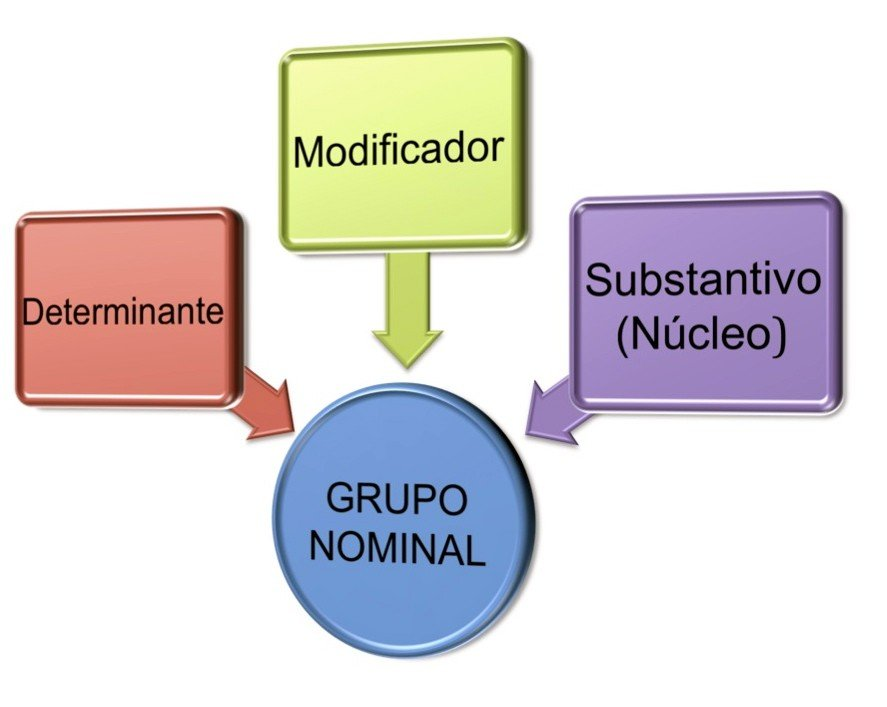
\includegraphics[width=0.65\textwidth]{images/grupo_nominal.jpg}
\end{frame}

%% --------------------------------------------------------

\begin{frame}{Exemplos de grupos nominais}

\begin{itemize}
    \item \textcolor{red}{An} \textcolor{blue}{expensive} \textcolor{bronze}{house}
    \item \textcolor{blue}{My} \textcolor{blue}{first} \textcolor{bronze}{day}
    \item \textcolor{bronze}{Cats} and \textcolor{bronze}{dogs}
    \item \textcolor{blue}{Your} \textcolor{bronze}{computer}
    \item \textcolor{red}{The} \textcolor{bronze}{chicken}
    \item \textcolor{red}{A} \textcolor{blue}{small} \textcolor{bronze}{car}
    \item \textcolor{blue}{Our} \textcolor{bronze}{study}
\end{itemize}

\vspace{1.5cm}

\hline

\textcolor{red}{Determinante} \hspace{2.5cm} \textcolor{blue}{Modificador} \hspace{2.5cm} \textcolor{bronze}{Núcleo}

\end{frame}

%% --------------------------------------------------------

\begin{frame}{Grupos nominais}

Um grupo nominal nos dá aquela estranha impressão que as frases em inglês são ao contrário
\begin{itemize}
    \item O núcleo sempre é a última estrutura do grupo nominal
    \item Desta forma, é normal fazermos a tradução da direita para a esquerda
\end{itemize}

\vspace{1cm}

\textbf{EN}: An environmentally responsible manufacturing company

\textbf{PT-BR}: Uma empresa de manufatura ambientalmente responsável

\vspace{0.5cm}

\textbf{EN}: The specially programmed volunteer vacations

\textbf{PT-BR}: As férias para voluntários especialmente programadas
\end{frame}

%% --------------------------------------------------------

\begin{frame}{Determinantes}

Um \textbf{determinante} é uma palavra que atua como identificador ou quantificador de substantivos ou grupos nominais
\begin{itemize}
    \item Artigos definidos e indefinidos
    \item Numerais cardinais e ordinais
    \item Pronomes indefinidos, demonstrativos, possessivos e distributivos
    \item ...
\end{itemize}

\vspace{0.5cm}

A seguir, veremos os principais determinantes utilizados na língua inglesa

\end{frame}

%% --------------------------------------------------------

\begin{frame}{Determinantes - Artigos}

\begin{minipage}{.54\textwidth}
Artigos são palavras que indicam algo
\begin{itemize}
    \item Definidos ou indefinidos
    \item Singular ou plural
\end{itemize}
\end{minipage}
\begin{minipage}{.44\textwidth}
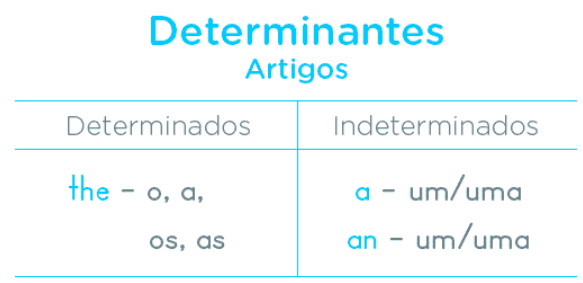
\includegraphics[width=\linewidth]{images/determinantes_artigos.png}
\end{minipage}

\vspace{0.5cm}

Bring \textbf{the} book when you finish with it.

Traga \textbf{o} livro quando você tiver terminado.

\vspace{0.2cm}

Elena gave me \textbf{a} medal for my accomplishments.

Elena me deu \textbf{uma} medalha pelas minhas conquistas.

\vspace{0.2cm}

We need \textbf{an} architect to design our house.

Nós precisamos de \textbf{um} arquiteto para projetar nossa casa.

\end{frame}

%% --------------------------------------------------------

\begin{frame}{Determinantes - Demonstrativos}

\begin{minipage}{.54\textwidth}
São utilizados para demonstrar ou indicar algo
\begin{itemize}
    \item Fazem referência a algo
\end{itemize}
\end{minipage}
\begin{minipage}{.44\textwidth}
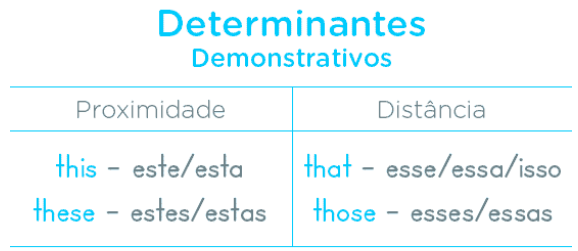
\includegraphics[width=\linewidth]{images/determinantes_demonstrativos.png}
\end{minipage}

\vspace{0.5cm}

Leonard told me that \textbf{those} are his dogs.

Leonard me disse que \textbf{aqueles} são seus cachorros.

\vspace{0.2cm}

Camila and Daniel go to \textbf{that} school around the corner.

Camila e Daniel vão para \textbf{aquela} escola virando a esquina.

\vspace{0.2cm}

I will use \textbf{these} green earrings.

Eu usarei \textbf{estes} brincos verdes.

\end{frame}

%% --------------------------------------------------------

\begin{frame}{Determinantes - Possessivos}

\begin{minipage}{.54\textwidth}
Indicam posse
\begin{itemize}
    \item Indicam o dono de algo
\end{itemize}

\vspace{0.5cm}

This is \textbf{my} new bike.

Esta é \textbf{minha} bicicleta nova.

\vspace{0.5cm}

The girls are going to \textbf{your} house.

As meninas estão indo para \textbf{sua} casa.

\end{minipage}
\begin{minipage}{.44\textwidth}
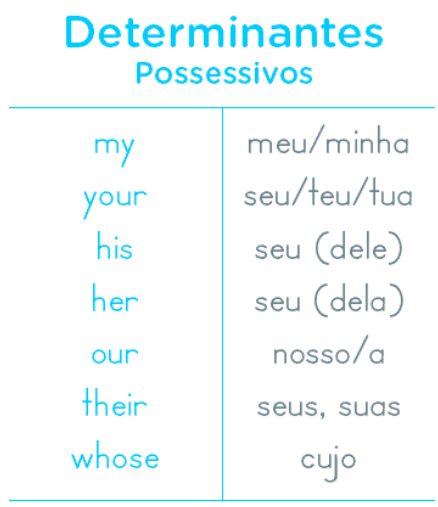
\includegraphics[width=\linewidth]{images/determinantes_possessivos.png}
\end{minipage}

\vspace{0.5cm}

I'm wearing \textbf{my} favorite shirt and \textbf{my brother’s} hat.

Eu estou usando \textbf{minha} camisa preferida e o chapéu do \textbf{meu} irmão.

\end{frame}

%% --------------------------------------------------------

\begin{frame}{Determinantes - Distributivos}

\begin{minipage}{.54\textwidth}
Fazem referência a um grupo de objetos
\begin{itemize}
    \item Pessoas, animais, objetos inanimados
    \item Distribuem ou dividem estes objetos
\end{itemize}

\vspace{0.5cm}

Elisa had \textbf{both} books.

Elisa tinha \textbf{ambos} livros.

\end{minipage}
\begin{minipage}{.44\textwidth}
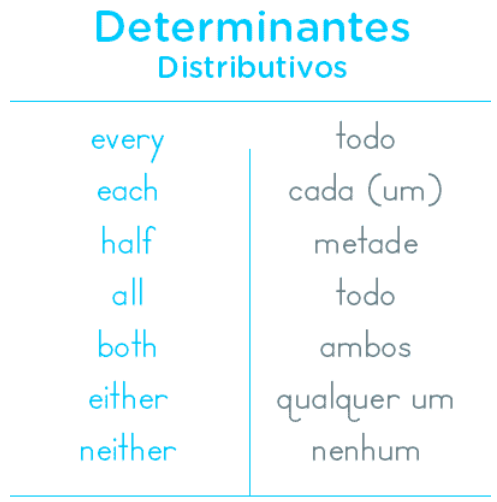
\includegraphics[width=\linewidth]{images/determinantes_distributivos.png}
\end{minipage}

\vspace{0.25cm}

The team could play in \textbf{either} field.

O time podia jogar em \textbf{qualquer um} dos campos.

\vspace{0.2cm}

You can talk to \textbf{all} of them.

Você pode conversar com \textbf{todos} eles.

\end{frame}

%% --------------------------------------------------------

\begin{frame}{Determinantes - Quantificadores}

\begin{minipage}{.54\textwidth}
Quantificam o núcleo
\begin{itemize}
    \item Indica a quantidade
\end{itemize}

\vspace{0.5cm}

She has been to \textbf{many} places this past year.

Ela esteve em \textbf{muitos} lugares este ano.

\vspace{0.25cm}

Maria has \textbf{enough} water in her backpack.

Maria tem água \textbf{suficiente} na sua mochila.

\end{minipage}
\begin{minipage}{.44\textwidth}
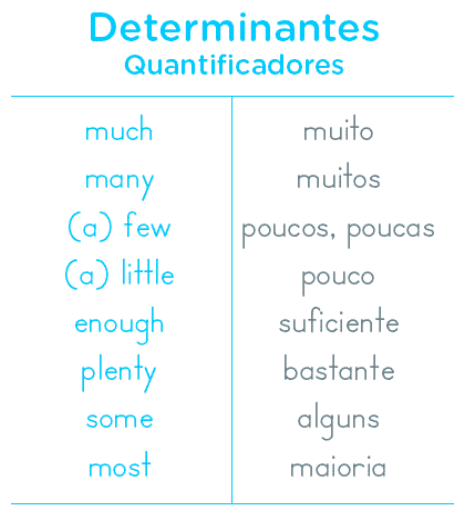
\includegraphics[width=\linewidth]{images/determinantes_quantificadores.png}
\end{minipage}

\vspace{0.5cm}

The boys have \textbf{some} books on the table.

Os meninos têm \textbf{alguns} livros sobre a mesa.

\end{frame}

%% --------------------------------------------------------

\begin{frame}{Determinantes - Diferença}

\begin{minipage}{.44\textwidth}
Exibem diferença em relação ao substantivo
\begin{itemize}
    \item Também podem indicar algo antagônico
\end{itemize}
\end{minipage}
\begin{minipage}{.54\textwidth}
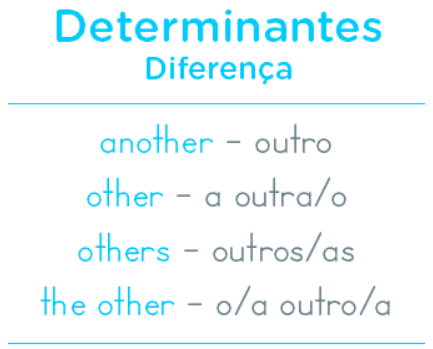
\includegraphics[width=\linewidth]{images/determinantes_diferenca.png}
\end{minipage}

\vspace{0.5cm}

I didn’t bring the green bag, I brought the \textbf{other} one.

Eu não trouxe a bolsa verde, eu trouxe a \textbf{outra}.

\vspace{0.15cm}

Fanny is not with Emily, she’s with her \textbf{other} friend.

Fanny não está com Emile, ela está com sua \textbf{outra} amiga.

\end{frame}

%% --------------------------------------------------------

\begin{frame}{Determinantes - Numerais}

\begin{minipage}{.49\textwidth}
Exprimem ordem ou quantidade
\begin{itemize}
    \item Cardinais
    \item Ordinais
\end{itemize}
\end{minipage}
\begin{minipage}{.49\textwidth}
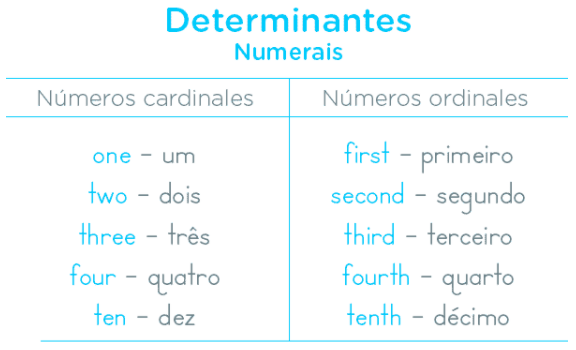
\includegraphics[width=\linewidth]{images/determinantes_numerais.png}
\end{minipage}

\vspace{0.5cm}

I slept with \textbf{two} blankets

Eu dormi com \textbf{dois} cobertores

\vspace{0.15cm}

He won the \textbf{first} prize!

Ele ganhou o \textbf{primeiro} prêmio!

\vspace{0.15cm}

Jordan has \textbf{three} black cat and \textbf{one} big dog 

Jordan tem \textbf{três} gatos pretos e \textbf{um} cachorro grande

\end{frame}

%% --------------------------------------------------------

\begin{frame}{Modificadores}

Um \textbf{modificador} é uma palavra que funciona como um adjetivo ou advérbio
\begin{itemize}
    \item Pode qualificar o substantivo (núcleo do grupo nominal)
\end{itemize}

\vspace{0.5cm}

Também existem diversos diferentes tipos de modificadores
\begin{itemize}
    \item Adjetivos
    \item Advérbios
    \item Casos possessivos
\end{itemize}
\end{frame}

%% --------------------------------------------------------

\begin{frame}{Modificadores - Adjetivos}

Um adjetivo é uma palavra que modifica um substantivo
\begin{itemize}
    \item Mesma função sintática que o adjetivo em português
    \item Denota uma característica 
    \item Qualifica ou delimita o substantivo
\end{itemize}

\vspace{0.5cm}

Lista dos adjetivos mais comuns (com tradução) \href{https://www.berlitz.com/pt-br/blog/60-adjetivos-em-ingles-para-ampliar-seu-vocabulario}{\beamergotobutton{Link}}

Lista mais completa com adjetivos \href{https://www.paperrater.com/page/lists-of-adjectives}{\beamergotobutton{Link}}

\end{frame}

%% --------------------------------------------------------

\begin{frame}{Modificadores - Advérbios}

Um advérbio, assim como um adjetivo, denota uma característica
\begin{itemize}
    \item Entretanto, ele não qualifica ou delimita o substantivo
    \item Ao invés disso, ele modifica ou exprime característica de
    \begin{itemize}
        \item Verbos
        \item Outros advérbios
        \item Adjetivos
        \item Em alguns casos, de sentenças inteiras!
    \end{itemize}
\end{itemize}

\vspace{0.5cm}

Um advérbio pode exprimir circunstâncias de

\begin{minipage}{.32\textwidth}
\begin{itemize}
    \item Tempo
    \item Modo
    \item Lugar
    \item Qualidade
\end{itemize}
\end{minipage}
\begin{minipage}{.33\textwidth}
\begin{itemize}
    \item Oposição
    \item Afirmação
    \item Negação
    \item Dúvida
\end{itemize}
\end{minipage}
\begin{minipage}{.32\textwidth}
\begin{itemize}
    \item Causa
    \item Intensidade
    \item Aprovação
    \item $\ldots$
\end{itemize}
\end{minipage}

\end{frame}

%% --------------------------------------------------------

\begin{frame}{Modificadores - Advérbios}

Pode-se enxergar um advérbio como uma resposta a uma pergunta
\begin{minipage}{.49\textwidth}
\begin{itemize}
    \item Quem?
    \item Quando?
    \item Como?
\end{itemize}
\end{minipage}
\begin{minipage}{.49\textwidth}
\begin{itemize}
    \item Quanto?
    \item Por quanto tempo?
    \item Com que frequência?
\end{itemize}
\end{minipage}

\vspace{0.5cm}

Exemplos de advérbios em sentenças

\begin{itemize}
    \item The elections are coming \textbf{soon}.
    \item They only shopped \textbf{locally}.
    \item They are \textbf{happily} married.
    \item The roads are very \textbf{steep}.
    \item He stopped by \textbf{briefly} to say hello.
    \item My daughter calls me \textbf{regularly}.
\end{itemize}
\end{frame}

%% --------------------------------------------------------

\begin{frame}{Modificadores - Advérbios}

Muitos advérbios são formados a partir de adjetivos
\begin{itemize}
    \item Acrescenta-se \textit{-ly} ao adjetivo
    \item Caso ele termine em \textit{-y}
    \begin{itemize}
        \item Troca-se o \textit{y} por \textit{i}
    \end{itemize}
\end{itemize}

\vspace{0.5cm}

\begin{itemize}
    \item Bold / Boldly (Corajosamente)
    \item Solid / Solidly (Solidamente, substancialmente)
    \item Heavy / Heavily (Fortemente)
    \item Interesting / Interestingly (Interessantemente)
    \item Necessary / Necessarily (Necessariamente)
\end{itemize}

\end{frame}

%% --------------------------------------------------------

\begin{frame}{Modificadores - Casos possessivos}

Utilizado para demonstrar posse
\begin{itemize}
    \item Declara que o sujeito (núcleo) é dono de algo
\end{itemize}

\vspace{0.25cm}

O caso possessivo é realizado acrescentando um \textbf{'s} ao substantivo
\begin{itemize}
    \item Ou somente o \textbf{'} se o substantivo já termina em \textbf{s}
    \item Caso existam dois substantivos, acrescenta-se somente ao último
\end{itemize}

\vspace{0.25cm}

Exemplos
\begin{itemize}
    \item This is \textbf{Mary’s} book. (Este é o livro da Mary.)
    \item \textbf{Bob and Jill’s} bedroom is a mess. (O quarto do Bob e da Jill está uma bagunça.)
    \item Those are \textbf{Ted’s} boots. (Aquelas são as botas do Ted.)
    \item \textbf{Chris’} apartment is huge! (O apartamento do Chris é imenso!)
\end{itemize}
\end{frame}

\end{document}